%% Mixed-Precision RISC-V SoC Architecture Diagram
%% Compile with: pdflatex architecture_diagram.tex
%%
\documentclass[border=10pt]{standalone}
\usepackage{tikz}
\usetikzlibrary{positioning, fit, arrows.meta, calc, shapes.geometric, backgrounds}
\usepackage{xcolor}

% Color palette
\definecolor{cpuBlue}{HTML}{2563EB}
\definecolor{cpuBlueLt}{HTML}{DBEAFE}
\definecolor{accelGreen}{HTML}{059669}
\definecolor{accelGreenLt}{HTML}{D1FAE5}
\definecolor{nvfp4Orange}{HTML}{D97706}
\definecolor{nvfp4OrangeLt}{HTML}{FEF3C7}
\definecolor{bf16Purple}{HTML}{7C3AED}
\definecolor{bf16PurpleLt}{HTML}{EDE9FE}
\definecolor{topGray}{HTML}{374151}
\definecolor{topGrayLt}{HTML}{F3F4F6}
\definecolor{busRed}{HTML}{DC2626}

\begin{document}
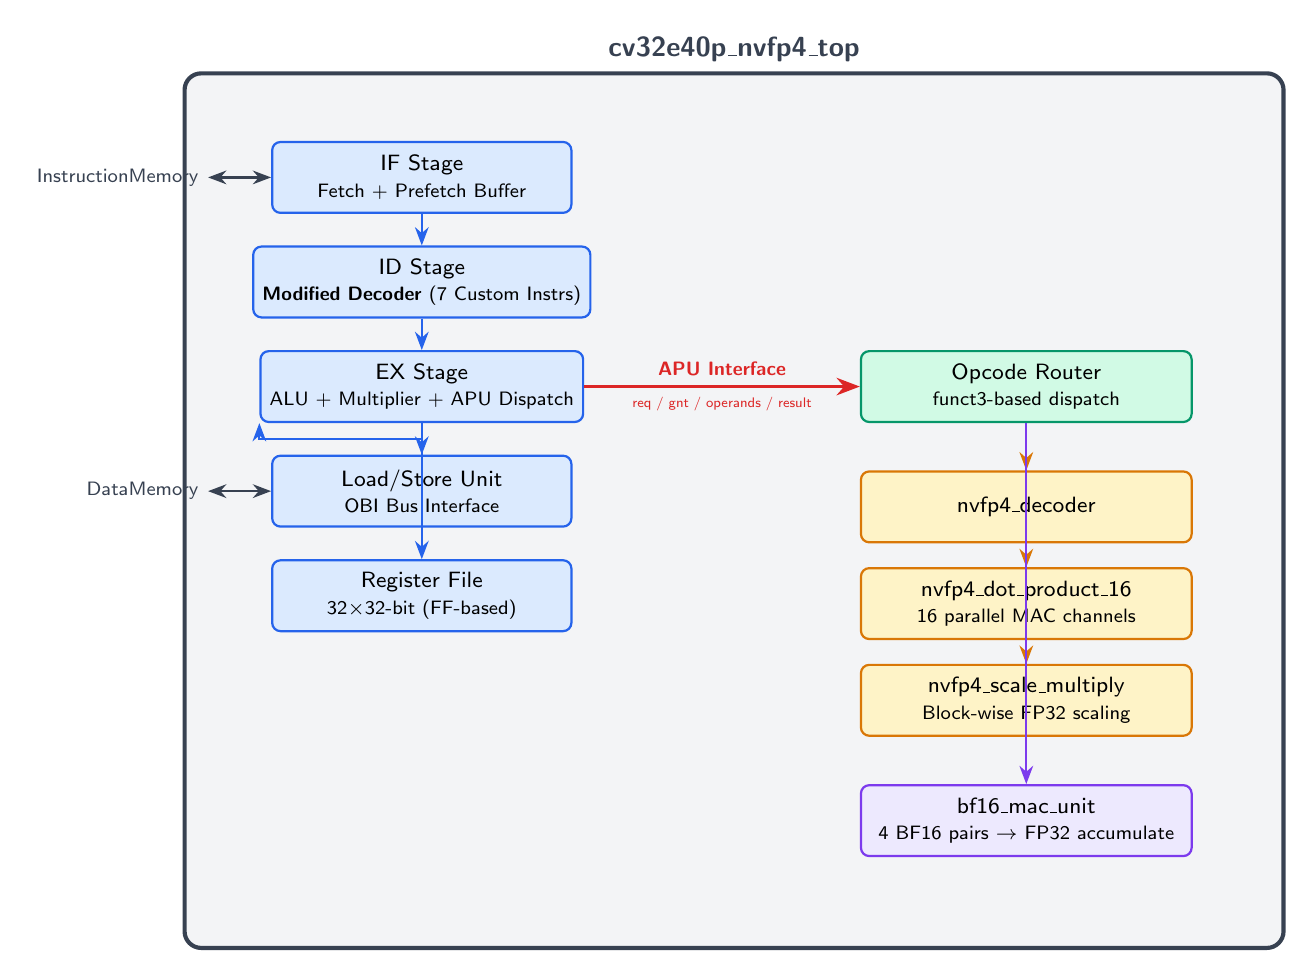
\begin{tikzpicture}[
    >=Stealth,
    node distance=0.4cm,
    block/.style={
        draw, rounded corners=3pt, minimum width=3.8cm, minimum height=0.9cm,
        font=\footnotesize\sffamily, align=center, thick
    },
    cpublock/.style={block, fill=cpuBlueLt, draw=cpuBlue},
    accelblock/.style={block, fill=accelGreenLt, draw=accelGreen},
    nvfp4block/.style={block, fill=nvfp4OrangeLt, draw=nvfp4Orange},
    bf16block/.style={block, fill=bf16PurpleLt, draw=bf16Purple},
    groupbox/.style={draw, rounded corners=6pt, thick, inner sep=8pt},
]

% ============================================
% CPU Pipeline (Left Side)
% ============================================
\node[cpublock] (if) {IF Stage\\{\scriptsize Fetch + Prefetch Buffer}};
\node[cpublock, below=of if] (id) {ID Stage\\{\scriptsize \textbf{Modified Decoder} (7 Custom Instrs)}};
\node[cpublock, below=of id] (ex) {EX Stage\\{\scriptsize ALU + Multiplier + APU Dispatch}};
\node[cpublock, below=of ex] (lsu) {Load/Store Unit\\{\scriptsize OBI Bus Interface}};
\node[cpublock, below=of lsu] (rf) {Register File\\{\scriptsize 32$\times$32-bit (FF-based)}};

% CPU group box
\begin{scope}[on background layer]
\node[groupbox, fill=cpuBlueLt!30, draw=cpuBlue, 
      fit=(if)(id)(ex)(lsu)(rf), 
      label={[font=\small\sffamily\bfseries, text=cpuBlue]above:cv32e40p\_core (RISC-V RV32IMC)}] (cpubox) {};
\end{scope}

% ============================================
% Accelerator Side (Right Side)
% ============================================
\node[accelblock, right=3.5cm of ex, minimum width=4.2cm] (router) {Opcode Router\\{\scriptsize funct3-based dispatch}};

% NVFP4 Accelerator
\node[nvfp4block, below=0.6cm of router, minimum width=4.2cm] (dec) {nvfp4\_decoder};
\node[nvfp4block, below=0.3cm of dec, minimum width=4.2cm] (dot) {nvfp4\_dot\_product\_16\\{\scriptsize 16 parallel MAC channels}};
\node[nvfp4block, below=0.3cm of dot, minimum width=4.2cm] (scale) {nvfp4\_scale\_multiply\\{\scriptsize Block-wise FP32 scaling}};

% NVFP4 group box
\begin{scope}[on background layer]
\node[groupbox, fill=nvfp4OrangeLt!40, draw=nvfp4Orange,
      fit=(dec)(dot)(scale),
      label={[font=\scriptsize\sffamily\bfseries, text=nvfp4Orange]above:NVFP4 Accelerator (4-bit)}] (nvfp4box) {};
\end{scope}

% BF16 MAC Unit
\node[bf16block, below=0.6cm of scale, minimum width=4.2cm] (bf16) {bf16\_mac\_unit\\{\scriptsize 4 BF16 pairs $\rightarrow$ FP32 accumulate}};

% BF16 group box
\begin{scope}[on background layer]
\node[groupbox, fill=bf16PurpleLt!40, draw=bf16Purple,
      fit=(bf16),
      label={[font=\scriptsize\sffamily\bfseries, text=bf16Purple]above:BF16 MAC Unit (16-bit)}] (bf16box) {};
\end{scope}

% Adapter group box
\begin{scope}[on background layer]
\node[groupbox, fill=accelGreenLt!30, draw=accelGreen,
      fit=(router)(nvfp4box)(bf16box),
      label={[font=\small\sffamily\bfseries, text=accelGreen]above:nvfp4\_apu\_adapter}] (adapterbox) {};
\end{scope}

% ============================================
% Top-level box
% ============================================
\begin{scope}[on background layer]
\node[groupbox, fill=topGrayLt, draw=topGray, line width=1.5pt,
      fit=(cpubox)(adapterbox),
      inner sep=16pt,
      label={[font=\normalsize\sffamily\bfseries, text=topGray]above:cv32e40p\_nvfp4\_top}] (topbox) {};
\end{scope}

% ============================================
% Connections
% ============================================

% CPU pipeline flow
\draw[->, thick, cpuBlue] (if) -- (id);
\draw[->, thick, cpuBlue] (id) -- (ex);
\draw[->, thick, cpuBlue] (ex) -- (lsu);
\draw[<->, thick, cpuBlue] (ex.south west) -- ++(0, -0.2) -| (rf.north);

% APU Interface (CPU → Adapter)
\draw[->, very thick, busRed] (ex.east) -- node[above, font=\scriptsize\sffamily\bfseries, text=busRed] {APU Interface} node[below, font=\tiny\sffamily, text=busRed] {req / gnt / operands / result} (router.west);

% Router to sub-units
\draw[->, thick, nvfp4Orange] (router.south) -- ++(0, -0.15) -| (dec.north);
\draw[->, thick, nvfp4Orange] (dec) -- (dot);
\draw[->, thick, nvfp4Orange] (dot) -- (scale);

\draw[->, thick, bf16Purple] (router.south) -- ++(0, -0.15) -| ($(bf16.north) + (0, 1.8)$) -- ($(bf16.north) + (0, 0)$);

% ============================================
% External interfaces (memory bus)
% ============================================
\node[font=\scriptsize\sffamily, text=topGray, left=0.8cm of if] (imem) {Instruction\\Memory};
\node[font=\scriptsize\sffamily, text=topGray, left=0.8cm of lsu] (dmem) {Data\\Memory};

\draw[<->, thick, topGray] (if.west) -- (imem.east);
\draw[<->, thick, topGray] (lsu.west) -- (dmem.east);

\end{tikzpicture}
\end{document}
